\documentclass[12pt,a4paper]{article}
\usepackage[utf8]{inputenc}
\usepackage[english]{babel}
\usepackage{amsmath}
\usepackage{amsfonts}
\usepackage{amssymb}
\usepackage{graphicx}

\usepackage{fullpage}

\usepackage{float}

\usepackage{tikz}
\usetikzlibrary{arrows,automata, positioning,calc,shapes.geometric}

\begin{document}

\section{Physical Design}
To solve the sokoban problem a robot capable of performing simple tasks concerned with moving the can and itself around the game map are needed.
The behaviours the robot should be able to perform define how the robot should be formed in order to accomplish its task of solving the sokoban problem.
Therefore first the capabilities of the robot are considered and how this is reflected in the robot design.


\subsection{System Behaviours}
The robot was decided to be build upon being able to execute simple behaviours.
The execution of the behaviours would then be controlled from the \textit{Brain},
this is illustrated in figure \ref{fig:behaviourSystem}.

% brain/behaviour diagram
\begin{figure}[H]
\center
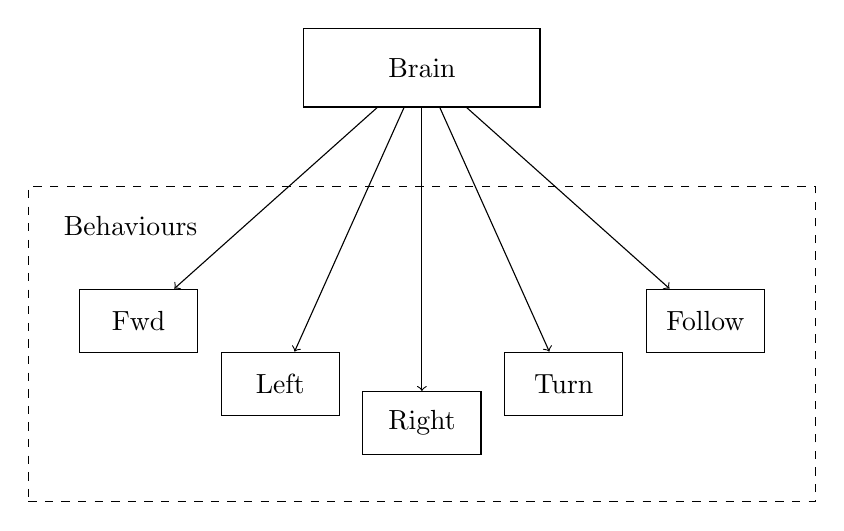
\begin{tikzpicture}[node distance=1cm]
%  behaviour box
\node[rectangle,draw,minimum width=10cm, minimum height=4cm, dashed, name=behaviour_box]  at (0,0) {};
\node[name=behaviour] at (-3.7,1.5) {Behaviours};

% Brain node 
\node[rectangle,draw,minimum width=3cm, minimum height=1cm, name=brain, above=of behaviour_box] {Brain};

% behaviours
\node[rectangle,draw,minimum width=1.5cm, minimum height=0.8cm, name=fwd] at (-3.6,0.3) {Fwd};
\node[rectangle,draw,minimum width=1.5cm, minimum height=0.8cm, name=left] at (-1.8,-0.5) {Left};
\node[rectangle,draw,minimum width=1.5cm, minimum height=0.8cm, name=right] at (0,-1.) {Right};
\node[rectangle,draw,minimum width=1.5cm, minimum height=0.8cm, name=turn] at (1.8,-0.5) {Turn};
\node[rectangle,draw,minimum width=1.5cm, minimum height=0.8cm, name=follow] at (3.6,0.3) {Follow};

% arrows inside 
\draw[->] (brain) -- (fwd) ;
\draw[->] (brain) -- (left) ;
\draw[->] (brain) -- (right) ;
\draw[->] (brain) -- (follow) ;
\draw[->] (brain) -- (turn) ;
\end{tikzpicture}
\caption{Overview of the systems behaviours.}
\label{fig:behaviourSystem}
\end{figure}

Here the central unit, the \textit{Brain} is responsible for finding the solution to the sokoban problem by invoking the five behaviours.
The \textit{Brain} is hence a combination of both the computer processing the map offline and the Lego-robot online when using the offline generated data to solve the puzzle.

The behaviours are defined in table \ref{tab:behaviourExplained} and based on dividing the behaviours into simple tasks which are easy to program.

\begin{table}[H]
\center
\begin{tabular}{c|l}
Behaviour & Description \\ \hline
Fwd & Makes the robot go straight ahead in the next intersection. \\
Left / Right & The robot turns left/right in the next intersection. \\
Turn & Turns the robot 180 degrees around in the next intersection. \\
Follow & Makes the robot follow the line till next intersection.
\end{tabular}
\caption{Behaviour table.}
\label{tab:behaviourExplained}
\end{table}

With these five behaviours the robot should then be able to navigate around the map and when a tomato can is encountered, push it to its destination.

\subsection{Physical Structure}

% img of robot (schematic)

\end{document}